\documentclass{article}
\usepackage{graphicx} % Required for inserting images
\usepackage{enumerate}
\usepackage{amsmath}
\usepackage{bm}
\usepackage[ruled,linesnumbered]{algorithm2e}

\def\T{\mathrm{T}}


\title{Greedy-based RBS maximum allowable current calculation method}
\author{3057761608 }
\date{March 2023}

\begin{document}

\maketitle

\section{Introduction}

% Battery energy storage systems(BESS) 被用在新能源汽车、风力发电站等场景中,为设备提供高品位电能的保存和释放。
Battery Energy Storage Systems (BESSs) are used to store and release high quality electrical energy in a timely manner in scenarios such as electric vehicles and wind power turbines.
A large number of individual battery cells are interconnected in groups by circuitry to form the main body of BESSs and achieve the required capacity and voltage for the application. 
However, the large number of cells also poses a challenge to the reliability of BESS: capacity and lifetime of the system depends mainly on the least healthy battery cells, known as the cask effect. 
As the multiple charge/discharge cycles of BESSs exacerbate the inconsistency of individual cells, the unhealthy batteries will appear early in operation.


% 【RBS的先进性、现状】
% Reconfigurable battery system(RBS) 解决固定电路电池组的 cask effect:系统的容量和寿命取决于状态最差的某些电池。
% 此外,不一致性也在系统运行中加剧恶化。
% 通过动态改变电路,调控或隔离不良电池,有助于提升系统整体可靠性。
% 但是,重构也增加了设计、分析和控制的难度。
% 当前,系统有成百上千的电池,平均每个电池由3~5个开关控制,形成了庞大的状态空间。
Reconfigurable Battery System (RBS), which can dynamically change the connections between batteries and switch between different circuit configurations as required, is expected to solve the above problem. 
Unlike fixed configurations, reconfigurable circuits have additional switches connected to battery cells in specific topological patterns. 
Series/parallel switching relationships and even the isolation of unhealthy batteries can be achieved by controlling the states of these switches (open or closed). 
From the point of view of the battery cells, RBS has a higher reliability than conventional configurable battery systems. 
However, it also increases the complexity of design and control.
Each battery in RBS is controlled by an average of 3 to 5 switches. When the system has hundreds or thousands of cells, there is a huge state space waits to solve.


% 【快速评估系统最大电流的作用和意义、文献现状】
% (一些典型结构、控制策略、评估)
% 快速评估系统最大允许电流在设计、分析和控制中起到重要作用。
% 对设计,系统的最大输出电流
% 对控制,应对故障,静态结构破坏
% 但是没有严谨研究最大电流。(直接说没有)
% del: 一些研究使用了过度的简化,不准;(具体文献?):led
% del: 只针对小数量的电池和特定的结构,不普适(具体文献,容易找到):led
The importance of the Maximum Allowable Current (MAC), defined as the maximum current that the system can output to external electrical equipment when the currents of all the batteries in the system do not exceed the specified value, is beginning to be recognised in RBS research. 
From the definition it can be seen that MAC determines the maximum output current of the RBS during normal operation at the design stage and of the reconfigured system when the failed batteries are isolated during the run-in phase. 
MAC is therefore one of the key indicators used in the study for the design and evaluation of RBSs.
% (#TODO: 一些考虑最大许用电流的构建结构的策略)
(TODO: Some literature on strategies for RBS that take MAC into account)
However, none of the existing literature on RBS provides a method for calculating the MAC.


% 【本文的主要内容和结构】
% 我们提出了快速估计RBS的算法,基于贪婪策略。填补了这一空白。
The purpose of this paper is to propose an effective and efficient algorithm based on the greedy search strategy to solve the MAC of RBSs. 
A mathematical model of MAC is constructed and the optimal solution is searched in the state space of switches using maximising the number of cells directly connected in parallel as the strategy.


% 文章组织:section 2,算法的框架和细节;section 3,案例,讨论和验证;section 4 总结。
This paper is organized as follows. 
Section II presents the mathematical model and the algorithm in detail.
Section III solves an example proposed in \cite{kimDESADependableEfficient2012}and discusses the results. 
Finally, Section IV provides concluding remarks and directions forjk future work.

\section{Method}
% \subsection{model building}

% Graph model has been uesd in the past to represent the connectivity of batteries in the RBS.
% In the study by He et al. \cite{heExploringAdaptiveReconfiguration2013} the batteries in system are represented as the vertices in the graph, and the connectivity between them are expressed as the edges.
% \begin{figure}[htbp]
%     \centering
%     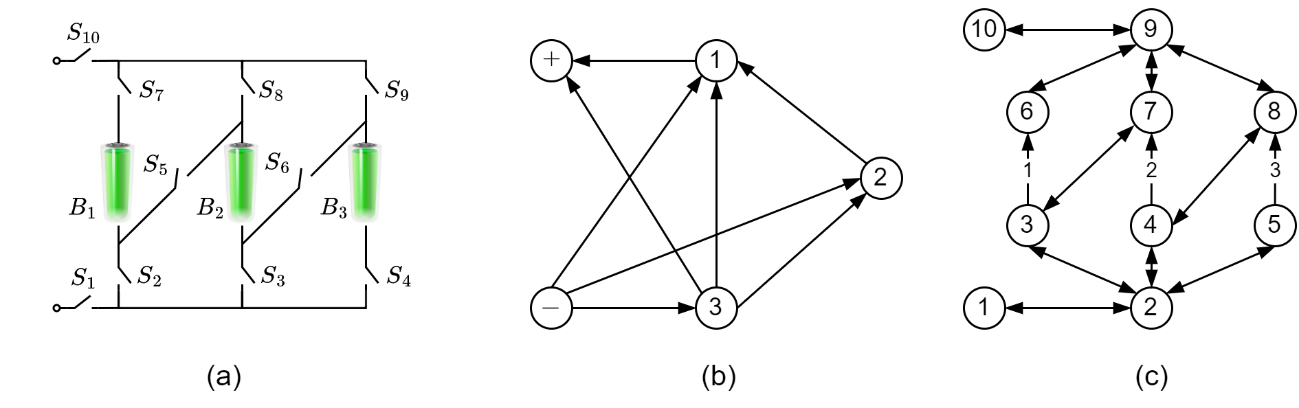
\includegraphics[width=\textwidth]{../attachments/graph_model.png} % #TODO: redraw figure c
%     \caption{A typical RBS architecture and its two common graph models. 
%             (a) RBS architecture \cite{kimDESADependableEfficient2012}, (b) graph model focused on connectivity \cite{heExploringAdaptiveReconfiguration2013}, (c) graph model used in this paper.}
%     \label{fig:graph_model}
% \end{figure}
% Figure \ref{fig:graph_model}(b) illustrates one example of the connectiviy model of a typical RBS architecture(Figure \ref{fig:graph_model}(a)).
% The additional vertices + and - in the figure represent the cathode and anode of the RBS, respectively, and the directed edges between the neighboring nodes represent the possible flows of current.
% However, this graph model % 写不下去了,我们的图模型能做的,He 的图模型基本也能做,甚至还要清晰

\subsection{circuit model}

A typical RBS circuit consists of battery cells and switches.
We first transform them into ideal components under reasonable assumptions to establish a processable circuit.
Then the circuit structure is described in matrix form and the related equations are given.


% 【电路,有向图,规定,假设】
% node,连接battery和switch,编号顺序
% edge,battery 或 switch,编号顺序
% 电池等效为恒压ub串内阻rb
% Ro,外电阻
% 关联矩阵
% x,开关状态,01变量
% 【模型,求解方法】
% 假设均一化,矩阵分块
% 在导纳矩阵非奇异的条件下
% 推导出输出电流Io和电池电流Ib
The normal equivalent circuit of a battery consists of a voltage source in series with a resistor, and a capacitor in parallel with another resistor to simulate the polarisation in batteries.
As the main aim of this research is to calculate the stable MAC offered by a given RBS architecture, only the steady-state behaviour of the circuit is taken into account, while transient effects are ignored in this research.
Thus, we equate the battery $i$ as a constant voltage source $u_{b,i}$ in series with a resistor $r_{b,i}$.
A binary variable $x_j$ is used to represent the state of the switch $j$: 0 and 1 mean open and closed respectively.
To simplify the calculation, the closed switch is considered as a resistor with a very small resistance value $r_s$, which will be treated as zero in the final result.
In the following derivation, the product of the conductance $1/r_s$ and the variable $x_j$ is used to characterize the state of the switch $j$.


Before obtaining the incidence matrix representing the structure of the circuit, a directed graph model $G(V,E)$ for the RBS is constructed in such a way that
\begin{enumerate}[(1)]
    \item the vertex set $V={v_1,v_2,\cdots,v_N}$ represents the nodes connecting batteries and/or switches, where $v_1$ and $v_N$ represent the anode and cathode of the RBS respectively;
    \item the directed edge set $E$ represents the output circuit, $N_b$ batteries and $N_s$ switches, corresponding set $E_o$, $E_b$ and $E_s$. The external electrical equipment in the output circuit is treated as one directed edge $v_n \to v_1$. The direction of the edge representing a battery is set to be from the anode to the cathode. For the edges representing switches, their directions are marked from the low node to the the high node. A negative value for the voltage drop or current solved on the edge means that the actual direction is opposite to that initially specified.
\end{enumerate}


Based on the above directed graph which has $N$ nodes and $1+N_b+N_s$ directed edges (1 refers to the output circuit), its incidence matrix $\bm{A}_{N\times (1+N_b+N_s)}$ is defined as
\begin{align}\label{eq:A}
    a_{ij}=
    \begin{cases}
        1,  & \text{edge  $j$ leaves vertex $i$},\\
        -1, & \text{edge $j$ enters vertex $i$},\\
        0,  & \text{otherwise}.
    \end{cases}
\end{align}
Since each column of $\bm{A}$ sums to zero, we delete the last line and use the reduced incidence matrix $\bm{A}_{(N-1)\times(1+N_b+N_s)}$ in the following calculation.
y splitting $E$ into $\{E_o, E_b, E_s\}$, $A$ is rewritten as follows
\begin{equation}
    \bm{A} = 
    \begin{bmatrix}
        \bm{A}_o & \bm{A}_b & \bm{A}_s
    \end{bmatrix}.
\end{equation}


$1+N_b+N_s$ edges' currents $\bm{I}_{(1+N_b+N_s)\times 1}$ and voltages $\bm{U}_{(1+N_b+N_s)\times 1}$, and $N-1$ nodes' voltages $\bm{U}_{n, (N-1)\times 1}$ have following relationships from Kirchhoffs law
\begin{align}\label{eq:Kirchhoffs_law}
    \begin{cases}
    \bm{A} \bm{I} = \bm{0}, \\
    \bm{U}        = \bm{A}^\T \bm{U}_n.
    \end{cases}
\end{align}
These directed edges are treated as generalized branches and expressed in matrix form as follows
\begin{equation}\label{eq:generalized_branches}
    \bm{I} = \bm{Y}\bm{X} \bm{U} - \bm{Y}\bm{X} \bm{U}_s +\bm{I}_s,
\end{equation}
where $\bm{I}$ and $\bm{U}$ are the column vectors about $1+N_b+N_s$ edges' current and voltage, respectively; 
$\bm{U}_s$ and $\bm{I}_s$ denote the source voltage and source current of the generalized branches, respectively;
$\bm{Y}$ is the admittance matrix of the circuit, and $\bm{X}$ is the state matrix defined as
\begin{equation}\label{eq:X}
    \bm{X} = diag(
        1,  
        \underbrace{1, \cdots, 1}_{N_b~\text{of}~1}, 
        \underbrace{1, 0 \cdots, 1}_{N_s~\text{of}~0/1}
    ).
\end{equation}


In addition to the equivalent circuit assumptions, we also assume that all batteries have the same internal resistance value $r_b$ and supply the same electric potential $u_s$ to simplify the model.
Then the output current $I_o$ and each battery's current $\bm{I}_b$ can be given by solving the simultaneous Equations \ref{eq:Kirchhoffs_law} and \ref{eq:generalized_branches} eventually.
Let
\begin{equation}\label{eq:Yn}
    \bm{Y}_n (\bm{X}) = \frac{1}{R_o} \bm{A}_o\bm{A}_o^\T + \frac{1}{r_b} \bm{A}_b\bm{A}_b^\T + \frac{1}{r_s}\bm{A}_s\bm{X}\bm{A}_s^\T,
\end{equation}
where $R_o$ is the equivalent resistance of the external circuit.
Then, if $\bm{Y}_n$ is an invertible matrix, 
\begin{align}
    I_o(\bm{X})      & = \frac{u_b}{R_o r_b} \bm{A}_o^\T \bm{Y}_n^{-1}(\bm{X}) \bm{A}_b \bm{I}_{N_b\times 1};\label{eq:I_o}\\
    \bm{I}_b(\bm{X}) & = \frac{u_b}{r_b^2}[\bm{A}_b^\T \bm{Y}_n^{-1}(\bm{X}) \bm{A}_b\bm{I}_{N_b \times 1}  -r_b \bm{I}_{N_b \times 1}],\label{eq:I_b}
\end{align}
where $\bm{I}_{N_b\times 1}$ is a column vector with all terms being one.


% 用外电流Ib比所有电池中最大电流max(Ib)之比,表征电路的最大许用输出。是电路结构本身的性质,与电池无关。电路的线性保证了。
% 目标问题转化为【数学形式】
% Max rate
% s.t.
We use the ratio of $I_o$ and $\max (\bm{I}_b)$ to characterize the allowable current for a given RBS architecture, denoted as $\eta$.
The $\eta$ reflects the ability of the RBS architecture itself to deliver current, regardliess of the battery cells used by the RBS.
Due to the linearity of the above circuit model, the output current will vary by the same multiple if the allowable current of all batteries varies by a certain multiple.
Our problem in RBS can be formulated as
\begin{align}
        & \max \eta \label{eq:max_eta}\\
    \mathrm{s.t.}\,\, & \eta = \frac{I_o}{\max (\bm{I}_b)}, \\
        & \max (\bm{I}_b) \leq I_m,
\end{align}
where $I_m$ is the maximum allowable current of the battery; $I_o$ and $\bm{I}_b$ can be calculated by Equations \ref{eq:I_o} and \ref{eq:I_b}.
The presence of the inverse matrix $\bm{Y}_n^{-1}$ prevents us from solving \ref{eq:max_eta} directly, especially when a large number of battery cells and switches are present in the system.
We therefore propose a greedy algorithm to solve this model.


\subsection{greedy solution}
% 使用贪心算法策略求解
% 【贪心策略】
% 电池i的最短路径,短指的是路径上电池数量最少
% 贪心策略,当系统中越多的电池被以最短路径联入电路,外电路电流越大。
% 短路,检查
% 组合,逐一
If the battery $i$ is connected to the anode $v_1$ and the cathode $v_N$ of the RBS by a certain line with the minimum number of battery cells on the path,
we call this path the shortest path ($SP_i$) for the battery $i$.
Since batteries can provide more total current when connected in parallel than in series, $SP_i$ is the path where battery $i$ contributes the most current to the system output.
Our solution greedily addresses the issue mentioned in the previous subsection: we greedily allow as many cells as possible to be connected to the overall circuit via $SP$.
We cannot guarantee that all cells will be connected into the circuit via their $SP$s at the same time, so we ues the following strategies to select $SP$s:
\begin{enumerate}[(1)]
    \item Recude the total number of $SP$s selected, when none of the valid circuits can be formed under the current number of $SP$s. 
    \item Calculate each combination on $SP$s one by one to obtain the $\eta$ under the given number of $SP$s. 
\end{enumerate}
We recommend using the dichotomy method to find the right number of selected $SP$s faster in our experience.


% 【总体流程(二分查找)】
% 对于给定结构和最大许用电流通过如下步骤得到:
% (伪代码开始)
% 通过图查找,深度优先,对每个电池找最短路径
% 以二分策略选择考察电池数量N_{select}
% 通过组合,形成C^{N_select}_{N_total}种方式,对于每种方式
% 	仅将选中的电池最短路径上的开关状态设置为1
% 	求解电流,公式
%	检查各电池电流,是否短路或超过电池的最大许用电流(否,break)
% 	给出外电路电流和所有电池电流的最大值,计算比率
% (伪代码结束)
% 电池电流Ib不超过ub/rb,未短路,合法(电池电流Ib受外电路Ro影响,考虑设一个固定值Ibmax,表示电池最大许用电流)
(TODO: this part is rubbish and wait to be revised)
The specific steps for calculating $\max \eta$ of a given RBS architecture $G(V,E)$ are described below:
\begin{enumerate}[\textbf{Step} 1:]
    \item Get $SP_i$(s) for each battery $i\in E_b$ using Depth-First Search.
    \item Get $\bm{A}$ of $G(V,E)$ by Equation \ref{eq:A}.
    \item Determine the number $N_{sel}$ of selected $SP$s: the initial value is $N_b$, after which the value is calculated by dichotomy.
    When $N_{sel}$ is no longer changing, go to \textbf{Step }8.
    \item Select $N_{sel}$ batteries from total $N_b$ for combination, and select the $SP$s of the selected cells for further combination. 
    The set of combinations about $SP_i$s of $N_{sel}$ batteries is denoted as $C_p(N_{sel})$. 
    For all $c_p$s in $C_p(N_{sel})$, determine whether the corresponding circuits meet the requirements and calculate the $\eta$s by the following \textbf{Step }5,6 and 7.
    \item For a $c_p\in C_p(N_{sel})$, let the switch $j$'s state variable be 1 if $j$ in the $c_p$; 0 otherwise. The $\bm{X}$ for the $c_p$ is further obtained by Equation \ref{eq:X}.
    If all $c_p$s in $C_p(N_{sel})$ have been selected, return to \textbf{Step }3.
    \item Calculate $\bm{Y}_n$ by \ref{eq:Yn} and determine whether the $Y_n$ is invertible.
    If so, perform the next step; otherwise, return to \textbf{Step }5 and select another $c_p$.
    \item Calculate output current $I_o$ and batteries's currents $\bm{I}_b$ by Equations \ref{eq:I_o} and \ref{eq:I_b}.
    Check if the max current of batteries $\max(\bm{I}_b)$ exceeds the permissible value $I_m$.
    If it does not exceed, calculate the ratio $I_o/\max(\bm{I}_b)$, i.e. $\eta$; otherwise, return to \textbf{Step }5 and select another $c_p$.
    \item Choose the largest one from all the calculated $\eta$s as the output.
\end{enumerate}


The pseudo-code of the algorithm is as follows:
\begin{algorithm}
    \caption{Get the max currents ratio of a certain RBS}\label{alg:eta_RBS}
    \KwData{Directed graph model $G(V,E)$ of the RBS}
    \KwResult{$\max \eta$}
    \For{$i \in E_b$}{$P_i \leftarrow \{path| \text{starts at $v_1$ and ends at $v_n$} \wedge \text{has the fewest edges $\in E_b$}\}$.}
    get $\bm{A}$ by Equation \ref{eq:A}\;
    \While{not yet determine $\max \eta$ }
        {
            $N_{sel} \leftarrow \text{number of selected $SP$s calculated by dichotomy}$\;
            $C_b    \leftarrow \text{set of all combinations of $N_{sel} $~batteries from $N_b$}$\;
            \For{$c_b \in C_b$}{
                $C_p  \leftarrow \text{set of all combinations of $p_{ij}\in P_i$ from $\{P_i|i\in c_b\}$} $\;
                \For{$c_p \in C_p$}{
                    $\bm{x}_s \leftarrow \text{list of all switches' state: $x_s[j]=1$ if $ j \in c_p$ else 0}$\;
                    $\bm{X} \leftarrow diag[1,1,\cdots,1,\bm{x}_s] $\;
                    get $\bm{Y}_n$ by Equation \ref{eq:Yn}\;
                    \eIf{$\bm{Y}_n$ is invertible}{
                        get $I_o$ by Equation \ref{eq:I_o}\;
                        get $\bm{I}_b$ by Equation \ref{eq:I_b}\;
                        \eIf{$\max(\bm{I}_b)\leq I_m$}{
                            $\eta \leftarrow I_o/\max(\bm{I}_b)$\;
                        }{break}
                    }{break}
                }
            }
        }
\end{algorithm}

\section{An example and discussions}
% 经典结构
% 建模
% 求解
% 正确性

\section{Conclusion}

\bibliographystyle{ieeetr}
\bibliography{../attachments/my_ref}

\end{document}
